\documentclass[a4paper,11pt]{article}
\usepackage[top = 2.5cm, bottom = 2.5cm, left = 2.5cm, right = 2.5cm]{geometry} 
\usepackage[spanish]{babel} %Castellanización
\usepackage[T1]{fontenc}
\usepackage[utf8]{inputenc}
\usepackage{amssymb, amsmath}
\usepackage{multirow}
\usepackage{booktabs}
\usepackage{graphicx}
\usepackage{setspace}
\setlength{\parindent}{0.25in}
\usepackage{float}
\usepackage{fancyhdr}
\usepackage[usenames]{color}
%\documentclass[tikz, border=2mm]{standalone}
\usepackage{karnaugh-map}
\usepackage{graphicx,caption}
\usepackage{verbatim}
\usepackage{hyperref}
\usepackage{algorithmic}
\usepackage{algorithm}
\usepackage{float}
\pagestyle{fancy}
\fancyhf{}

\lhead{\footnotesize INF221: Informe Tarea 2}%
\rhead{\footnotesize CA CS JS - P200}
\cfoot{\footnotesize \thepage} 

\begin{document}


%%%%%%%%%%%%%%%%%%%%%%%%%%%%%%%%%%%%%%%%%%%%%%%%
%%%%%%%%%%%%%%%%%%%%%%%%%%%%%%%%%%%%%%%%%%%%%%%%

\thispagestyle{empty} % This command disables the header on the first page. 

  \begin{minipage}{.2\linewidth}
    \begin{flushleft}
      
\includegraphics[height = 1.5cm]{Imagenes/UTFSM.jpg}
    \end{flushleft}
  \end{minipage}
  \hfill
  \begin{minipage}{.7\linewidth}
    \begin{flushright}
        Universidad Técnica Federico Santa María \\
        Departamento de Informática\\
        INF221 - Algoritmos y Complejidad\\
    \end{flushright}
  \end{minipage}
%\begin{center}
%    \hrule
%\end{center}

\vfill % Now we want to add some vertical space in between the line and our title.
\begin{center}
	{\Large Informe Tarea 2\\}
	{\huge Comparación de Algoritmos de Multiplicación de Matrices\\}
	\vspace{.5cm}
	\hrule
	\vspace{.5cm}
        % YOUR NAMES GO HERE
    {\large Constanza Alvarado V.} - constanza.alvaradov@usm.cl - Rol 201973521-7\\
    {\large Catalina Sierra H.} - catalina.sierrah@usm.cl - Rol 201973557-8\\
	{\large José Southerland S.} - jose.southerland@usm.cl - Rol 201973526-8\\
	
\end{center}
\vfill
\newpage
\section{Introducción}
En el presente informe se realizará una comparación del Algoritmo de Strassen y el Algoritmo Clásico de resolución de Matrices, con la finalidad de poder analizar sus tiempos de ejecución experimentando con distintos valores de $n$ y comparándolos con sus valores téoricos $\Theta(n^{2,81})$ y $\Theta(n^3)$ respectivamente.
\section{Desarrollo}
Para realizar las comparaciones, se crearon dos archivos en lenguaje Python: \texttt{strassen.py} y \texttt{tradicional.py}, que tienen implementados los algoritmos de Strassen y el Clásico respectivamente. Además, se crearon 9 archivos \texttt{.txt} que contienen distintas matrices de tamaño $n\times n$ con valores entre 0 y 9. Los archivos \texttt{.py} piden como input el número del caso que se desea probar; los resultados son mostrados por pantalla junto con el tiempo de ejecución que al programa le tomó calcular la multiplicación.\\

Inicialmente se había creado un archivo \texttt{strassen.py} donde el algoritmo se encontraba implementado usando la librería \texttt{numpy}. Se decidió mantener dicho archivo bajo el nombre de \texttt{strassenNumpy.py}, con la mera finalidad de poder tener otro punto de vista en el informe. \textbf{La implementación válida (sin librerías aparte de \texttt{time} y \texttt{sys}) es la del archivo \texttt{strassen.py}.}

\section{Resultados}

A continuación se muestran los tiempos de ejecución obtenidos:
\begin{table}[h]
\centering
\begin{tabular}{|l|l|l|l|}
\hline
\textbf{Matriz $n$} & \textbf{Tradicional [s]} & \textbf{Strassen sin numpy [s]} & \textbf{Strassen con numpy [s]} \\ \hline
2                                         & 0,0000057                                         & 0,00015                                & 0,00034                       \\ \hline
5                                         & 0,000042                                          & 0,000065                               & 0,000019                      \\ \hline
15                                        & 0,0010                                            & 0,00035                                & 0,000037                      \\ \hline
30                                        & 0,018                                             & 0,0084                                 & 0,0021                        \\ \hline
50                                        & 0,053                                             & 0,016                                  & 0,0054                        \\ \hline
100                                       & 0,18                                              & 0,11                                   & 0,049                         \\ \hline
200                                       & 1,49                                              & 0,84                                   & 0,39                          \\ \hline
500                                       & 20,36                                             & 10,44                                  & 1,26                          \\ \hline
1000                                      & 156,37                                            & 74,60                                  & 9,97                          \\ \hline
\end{tabular}
\end{table}\\
  \begin{minipage}{\linewidth}
      \centering
      \begin{minipage}{0.48\linewidth}
          \begin{figure}[H]
              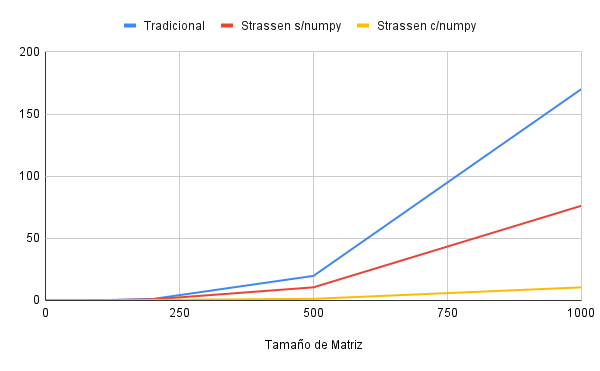
\includegraphics[width=\linewidth]{Imagenes/graph3.png}
              \caption{Gráfica con resultados obtenidos.}
          \end{figure}
      \end{minipage}
      \hspace{0.05\linewidth}
      \begin{minipage}{0.42\linewidth}
          \begin{figure}[H]
              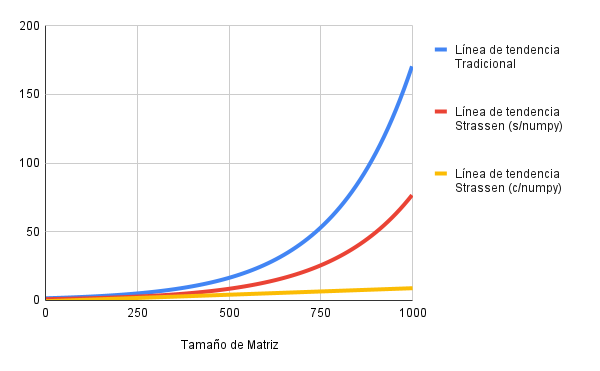
\includegraphics[width=\linewidth]{Imagenes/graph4.png}
              \caption{Gráfica con línea de tendencia exponencial de los datos obtenidos.}
          \end{figure}
      \end{minipage}
  \end{minipage}

\section{Conclusión}
A partir de los casos probados en ambos algoritmos, se puede concluir que sus tiempos de ejecución son exponenciales. Sin embargo, el Algoritmo de Strassen tiene una tendencia exponencial menor que el Algoritmo Clásico. Esto se puede notar de mejor forma en los casos donde la matriz tenía tamaño 500 y 1000. Para dichos casos, el Algoritmo Clásico dispara su tiempo de ejecución, mientras que el de Strassen aumenta pero en menor medida.\\

Paralelamente, el Algoritmo de Strassen implementado con \texttt{numpy} logra un tiempo mejor que las otras implementaciones. Esto es posible gracias a que \texttt{numpy} ofrece una forma de asignar matrices de manera más eficiente a la implementada manualmente.\\

Finalmente, es posible decir que se cumple lo mostrado teóricamente: el tiempo de ejecución de Strassen $\Theta(n^{2,81})$ es exponencial (tanto con o sin \texttt{numpy}), pero menor que el tiempo del Algoritmo Clásico ($\Theta(n^3)$). Para casos pequeños la diferencia es prácticamente imperceptible, pero desde los 500 casos en adelante toma muchísima importancia para obtener una solución más rápidamente.
\vfill
\vspace{.5cm}
\hrule
\vspace{.5cm}
\begin{thebibliography}{X}
\bibitem{Libro} \textsc{Arroyuelo D.} Algoritmos Discretos: Análisis y Diseño, Capítulo 11.
\bibitem{Geek} \textsc{Geeks for Geeks} Divide and Conquer: Strassen's Matrix Multiplication. \url{https://www.geeksforgeeks.org/strassens-matrix-multiplication/}
\end{thebibliography}

\end{document}